\chapter{HASIL DAN PEMBAHASAN}
\label{chap:hasildanpembahasan}

\section{Hasil Eksperimen}
\label{sec:hasilpengujian}

Pada bagian ini, kami akan membahas hasil eksperimen yang dilakukan
untuk menjawab rumusan masalah yang diajukan dalam penelitian ini.

\subsection{Lingkungan Pengujian}
\label{subsec:lingkunganpengujian}

Untuk menjawab rumusan masalah yang diajukan oleh penelitian ini,
kami melakukan eksperimen pada aplikasi \emph{benchmark}
DISC yang telah ada, yang diadaptasi dari penelitian sebelumnya
tentang \emph{debugging} dan pengujian aplikasi DISC. \emph{Benchmark}
ini merupakan campuran dari alur kerja \emph{big data} yang
terinspirasi dari SQL dan dunia nyata. Aplikasi-aplikasi
ini juga dilengkapi dengan kesalahan yang sudah disuntikkan
sebelumnya yang mewakili \emph{bug} dunia nyata. Secara total,
kami menjalankan eksperimen pada 16 aplikasi \emph{benchmark}
DISC yang bermasalah. Aplikasi-aplikasi ini dilengkapi
dengan skrip pembuatan data yang memungkinkan data
dihasilkan dengan faktor skala, mirip dengan
\emph{benchmark} TPC-DS. Kami menggunakan laptop standar
untuk menerapkan Apache Spark 2.0.0 karena Titian
awalnya dirancang untuk Apache Spark 2.0.0. Namun,
FISUM sepenuhnya kompatibel dengan versi terbaru dari
Spark karena tidak memerlukan instrumen apa pun dalam
kode sumber Apache Spark. 

Berikut adalah deskripsi dari ke 16 aplikasi \emph{benchmark}
yang digunakan dalam penelitian ini:
\begin{enumerate}
      \item \emph{\textbf{Age Analysis}} \\
            Program \emph{age analysis} digunakan untuk mengklasifikasikan penduduk di sebuah area dengan kode pos "90024" sesuai dengan umur mereka. 
            Dalam program ini, Titian diaplikasikan untuk mendeteksi input yang memiliki data penduduk yang memiliki umur lebih dari 50.
            Adapun contoh dataset yang digunakan dapat 
            dilihat pada Tabel \ref{tb:ageanalysisdataset}.

            \begin{longtable}{|c|c|c|}
                  \caption{Contoh Dataset Age Analysis.}
                  \label{tb:ageanalysisdataset} \\
                  \hline
                  \rowcolor[HTML]{C0C0C0}
                  \textbf{Kode Pos} & \textbf{Umur} & \textbf{Jumlah} \\
                  \hline
                  90024 & 20 & 1000 \\
                  90024 & 30 & 2000 \\
                  90024 & 159 & 3000 \\
                  \hline
            \end{longtable}
      
      \item \emph{\textbf{Commute Type}} \\
            Program \emph{commute type} menggunakan dataset berupa kode pos area A, kode pos area B, jarak, serta waktu yang ditempuh. Selanjutnya, program akan mengolah jarak dan waktu menjadi kecepatan yang terjadi dalam menempuh perjalanan dari area A ke B. Dari data kecepatan tersebut, program akan mengklasifikasikan ke dalam tiga kategori, yaitu sebagai berikut:
            \begin{itemize}
                  \item kecepatan $ > $ 40 = \emph{car}
                  \item kecepatan $ > $ 15 = \emph{public}
                  \item kecepatan $ \leq $ 15 = \emph{on foot}
            \end{itemize}
            Namun, dari ketiga kategori tersebut, untuk kecepatan $ > $ 100 dikategorikan sebagai kesalahan input karena mobil tidak akan melebihi batas kecepatan tersebut.
            Adapun contoh dataset yang digunakan dapat 
            dilihat pada Tabel \ref{tb:commutetypedataset}.

            \begin{longtable}{|c|c|c|c|c|}
                  \caption{Contoh Dataset Commute Type.}
                  \label{tb:commutetypedataset} \\
                  \hline
                  \rowcolor[HTML]{C0C0C0}
                  \textbf{\#} & \textbf{Kode Pos A} & \textbf{Kode Pos B} & \textbf{Jarak} & \textbf{Waktu} \\
                  sr & 90002 & 90017 & 1501 & 100 \\
                  sr & 90098 & 90077 & 2106 & 37 \\
                  sr & 90079 & 90009 & 7009 & 116 \\
                  \hline
            \end{longtable}

      \item \emph{\textbf{Commute Type Full}} \\
      % sr,90002,90017,1501,100
      % sr,90098,90077,2106,37
      % sr,90079,90009,7009,116
            Program \emph{commute type full} menggunakan 2 dataset, yaitu \emph{trips} dan \emph{locations}. Dataset \emph{trips} berupa kode pos area A, kode pos area B, jarak, serta waktu yang ditempuh. Sedangkan, dataset kedua yang digunakan adalah \emph{locations}, dataset ini berisi lokasi dari sebuah kode pos. Selanjutnya, program akan menggabungkan kedua dataset apabila ada kesamaan pada kode pos. Kemudian, program akan mengolah jarak dan waktu menjadi kecepatan yang terjadi dalam menempuh perjalanan dari kota A ke B. Dari data kecepatan tersebut, program akan mengklasifikasikan ke dalam tiga kategori, yaitu sebagai berikut:
            \begin{itemize}
                  \item kecepatan $ > $ 40 = \emph{car}
                  \item kecepatan $ > $ 15 = \emph{public}
                  \item kecepatan $ \leq $ 15 = \emph{on foot}
            \end{itemize}
            Pada program ini, Titian bekerja untuk mendeteksi input yang dianggap salah, yaitu yang memiliki ID lokasi kurang dari sama dengan 1000.
            Adapun contoh dataset yang digunakan dapat 
            dilihat pada Tabel \ref{tb:commutetypefulldataset}.

            \begin{longtable}{|c|c|c|c|c|}
                  \caption{Contoh Dataset Commute Type Full.}
                  \label{tb:commutetypefulldataset} \\
                  \hline
                  \rowcolor[HTML]{C0C0C0}
                  \textbf{\#} & \textbf{Kode Pos A} & \textbf{Kode Pos B} & \textbf{Jarak} & \textbf{Waktu} \\
                  sr & 90002 & 90017 & 1501 & 100 \\
                  sr & 90098 & 90077 & 2106 & 37 \\
                  sr & 90079 & 90009 & 7009 & 116 \\
                  \hline
            \end{longtable}
      
      \item \emph{\textbf{Customers}} \\
      % s"""$oid,$cid,$time,$item"""
      % order651,888,78895039,item797864327
      % order515,481,1701910512,item765935155
      % order531,24,1171869537,item354502894
            Program \emph{customers} akan mengolah dua dataset, yaitu dataset \emph{customers\_data} dan \emph{orders\_data}. Kedua dataset ini akan digabungkan apabila memiliki kesamaan data dan akan menganalisis customer mana yang setidaknya sudah membuat 3 kali pembelian dalam jangka waktu yang sudah ditentukan. Dalam program ini, Titian hanya mencari input data yang memiliki order ID kurang dari 100 dan dinyatakan sebagai input yang salah.
            Adapun contoh dataset yang digunakan dapat 
            dilihat pada Tabel \ref{tb:customersdataset}.

            \begin{longtable}{|c|c|c|c|}
                  \caption{Contoh Dataset Customers.}
                  \label{tb:customersdataset} \\
                  \hline
                  \rowcolor[HTML]{C0C0C0}
                  \textbf{ID Order} & \textbf{ID Pelanggan} & \textbf{Waktu} & \textbf{Item} \\
                  \hline
                  order651 & 888 & 78895039 & item797864327 \\
                  order515 & 481 & 1701910512 & item765935155 \\
                  order531 & 24 & 1171869537 & item354502894 \\
                  \hline
            \end{longtable}
            
      \item \emph{\textbf{Delays}} \\
      % s"""$tripId,$a,$d,$r"""
      % trip63811,2128804415,1221732780,route56
      % trip46102,1777873050,482274628,route49
      % trip38403,140174683,1960456261,route64
            \emph{Delays} adalah program yang digunakan untuk mencari data bus yang mengalami keterlambatan (\emph{delay}). Dataset yang digunakan ada 2, yaitu \emph{dataStation1} dan \emph{dataStation2}. Kedua dataset ini memiliki waktu keberangkatan dan tiba dari setiap ID perjalanan. Kemudian, kedua dataset digabungkan apabila memiliki kesamaan data. Selanjutnya, program akan menghitung keterlambatan dari waktu keberangkatan dan tiba dari setiap elemen. Dalam program ini, Titian diterapkan untuk mencari input data yang memiliki waktu keberangkatan lebih besar daripada waktu tiba, karena dinyatakan sebagai ketidakmungkinan dalam kasus nyata.
            Adapun contoh dataset yang digunakan dapat 
            dilihat pada Tabel \ref{tb:delaysdataset}.

            \begin{longtable}{|c|c|c|c|}
                  \caption{Contoh Dataset Delays.}
                  \label{tb:delaysdataset} \\
                  \hline
                  \rowcolor[HTML]{C0C0C0}
                  \textbf{ID Perjalanan} & \textbf{Waktu Berangkat} & \textbf{Waktu Tiba} & \textbf{Rute} \\
                  \hline
                  trip63811 & 2128804415 & 1221732780 & route56 \\
                  trip46102 & 1777873050 & 482274628 & route49 \\
                  trip38403 & 140174683 & 1960456261 & route64 \\
                  \hline
            \end{longtable}

      \item \emph{\textbf{Delivery Faults}} \\
      % s"""$did,$cid,$vend,$rating"""
      % dlvry96998,cust43114,vend65077,5
      % dlvry16209,cust64119,vend8516,5
      % dlvry89647,cust10882,vend3328,5
            \emph{Delivery Faults} adalah program yang dapat mencari pengiriman mana yang buruk dari rating yang dimilikinya. Titian diterapkan dalam program ini untuk mendeteksi input yang memiliki rating lebih dari 5.
            Adapun contoh dataset yang digunakan dapat 
            dilihat pada Tabel \ref{tb:deliveryfaultsdataset}.

            \begin{longtable}{|c|c|c|c|}
                  \caption{Contoh Dataset Delivery Faults.}
                  \label{tb:deliveryfaultsdataset} \\
                  \hline
                  \rowcolor[HTML]{C0C0C0}
                  \textbf{ID Pengiriman} & \textbf{ID Pelanggan} & \textbf{ID Vendor} & \textbf{Rating} \\
                  \hline
                  dlvry96998 & cust43114 & vend65077 & 5 \\
                  dlvry16209 & cust64119 & vend8516 & 5 \\
                  dlvry89647 & cust10882 & vend3328 & 5 \\
                  \hline
            \end{longtable}

      \item \emph{\textbf{External Call}} \\
      % Teks
      % This is a sentence
      % This not a sentence
      % This is a word
      % My name is black
      % I am a student
            Program \emph{external call} memiliki tujuan untuk mencari kata yang sering muncul dalam suatu dataset, cara kerjanya adalah menjumlahkan setiap kata yang sama, kemudian apabila kata tersebut muncul lebih dari 1 maka dinyatakan sebagai kata yang sering muncul. Dalam program ini, Titian hanya akan melacak data yang jarang muncul yaitu yang memiliki jumlah kemunculan kurang dari atau sama dengan 1.
            Adapun contoh dataset yang digunakan dapat 
            dilihat pada Tabel \ref{tb:externalcalldataset}.

            \begin{longtable}{|c|}
                  \caption{Contoh Dataset External Call.}
                  \label{tb:externalcalldataset} \\
                  \hline
                  \rowcolor[HTML]{C0C0C0}
                  \textbf{Teks} \\
                  \hline
                  This is a sentence \\
                  This not a sentence \\
                  This is a word \\
                  My name is black \\
                  I am a student \\
                  \hline
            \end{longtable}

      \item \emph{\textbf{Find Salary}} \\
      % $522224
      % $415728
      % $501565
      % $820638
            \emph{Find salary} menggunakan satu data set yang berisi nominal gaji setiap orang, Program ini akan mencari gaji yang kurang dari 300. Kemudian, Titian diterapkan hanya untuk mendeteksi gaji yang lebih besar atau sama dengan 300.
            Adapun contoh dataset yang digunakan dapat 
            dilihat pada Tabel \ref{tb:findsalarydataset}.

            \begin{longtable}{|c|}
                  \caption{Contoh Dataset Find Salary.}
                  \label{tb:findsalarydataset} \\
                  \hline
                  \rowcolor[HTML]{C0C0C0}
                  \textbf{Gaji} \\
                  \hline
                  \$522224 \\
                  \$415728 \\
                  \$501565 \\
                  \$820638 \\
                  \hline
            \end{longtable}

      \item \emph{\textbf{Flight Distance}} \\
      % s"""$airportCode,$airportName,$airportName2,$long,$lat,$continent"""
      % LAX,2n8Hga8ICV,MpQ4TQZrHs,151.3466,-68.5339,PRkqAcg4rZ
      % LAS,hOvx8HlmGI,ke7IhMxWmx,123.0983,5.819,zQ6Zrv9bgQ
      % LAS,AJSAZYp44p,lJW9lm2npx,135.2637,-25.0603,Fter9EB1Vd
      % LAS,3L4mwHv6Wr,pkUt6axm1Y,176.4615,23.2344,wcb4CeYYo7
      % LAS,eRUZDr9FqE,XXuxIq7gGT,-134.0949,10.8214,SxtFuOA1xS
            Program \emph{flight distance} adalah program yang dapat mengolah data dari dua dataset, yaitu \emph{flights\_data} dan \emph{airports\_data}, yang mana hasil akhirnya adalah akan mengetahui jarak dari keberangkatan dan tiba dari setiap penerbangan. 
            Terdapat banyak input yang berupa lokasi bandara, kami gunakan input yang memiliki lokasi berkode "LAS" dan "LAX" sebagai input yang salah. Kemudian, input tersebut akan dilacak dengan Titian.
            Adapun contoh dataset yang digunakan dapat 
            dilihat pada Tabel \ref{tb:flightdistancedataset}.

            \begin{longtable}{|p{0.12\linewidth}|p{0.17\linewidth}|p{0.17\linewidth}|c|c|c|}
                  \caption{Contoh Dataset Flight Distance.}
                  \label{tb:flightdistancedataset} \\
                  \hline
                  \rowcolor[HTML]{C0C0C0}
                  \raggedright{\textbf{Kode Bandara}} & \raggedright{\textbf{Nama Bandara Asal}} & \raggedright{\textbf{Nama Bandara Tujuan}} & \textbf{Long} & \textbf{Lat} & \textbf{Benua} \\
                  \hline
                  LAX & 2n8Hga8ICV & MpQ4TQZrHs & 151.3466 & -68.5339 & PRkqAcg4rZ \\
                  LAS & hOvx8HlmGI & ke7IhMxWmx & 123.0983 & 5.819 & zQ6Zrv9bgQ \\
                  LAS & AJSAZYp44p & lJW9lm2npx & 135.2637 & -25.0603 & Fter9EB1Vd \\
                  LAS & 3L4mwHv6W & pkUt6axm1Y & 176.4615 & 23.2344 & wcb4CeYYo7 \\
                  LAS & eRUZDr9FqE & XXuxIq7gGT & -134.0949 & 10.8214 & SxtFuOA1xS \\
                  \hline
            \end{longtable}
            
      \item \emph{\textbf{Income Aggregation}} \\
      % \item  s"""$zip,$age,$r"""
      % 90084,11,9248
      % 90080,12,6140
      % 90014,15,1199
      % 90031,53,7558
      % 90017,17,7820
            \emph{Income aggregation} menggunakan dataset yang terdiri dari kode pos, umur, dan jumlah income. Program ini digunakan untuk mengklasifikasikan income masing-masing orang dari umurnya. Lalu, Titian akan digunakan untuk melacak asal usul data yang memiliki kode pos 90024.
            Adapun contoh dataset yang digunakan dapat 
            dilihat pada Tabel \ref{tb:incomeaggregationdataset}.

            \begin{longtable}{|c|c|c|}
                  \caption{Contoh Dataset Income Aggregation.}
                  \label{tb:incomeaggregationdataset} \\
                  \hline
                  \rowcolor[HTML]{C0C0C0}
                  \textbf{Kode Pos} & \textbf{Umur} & \textbf{Pendapatan} \\
                  \hline
                  90024 & 11 & 9248 \\
                  90080 & 12 & 6140 \\
                  90014 & 15 & 1199 \\
                  90031 & 53 & 7558 \\
                  90017 & 17 & 7820 \\
                  \hline
            \end{longtable}

      \item \emph{\textbf{Inside Circle}} \\
      % s"""$x,$y,$r"""
      % 49,26,711
      % 7,26,1870
      % 79,62,845
      % 64,65,1768
      % 2,45,611
            \emph{Inside circle} digunakan untuk menghitung data 3 bilangan random untuk memastikan apakah bilangan x dan y ada dalam radius z. Kegagalan atau kesalahan input yang akan dicari dalam program ini adalah data yang memiliki ukuran x dan y yang berada di luar radius z, yang mana tidak ada di dalam lingkaran.
            Adapun contoh dataset yang digunakan dapat 
            dilihat pada Tabel \ref{tb:insidecircledataset}.

            \begin{longtable}{|c|c|c|}
                  \caption{Contoh Dataset Inside Circle.}
                  \label{tb:insidecircledataset} \\
                  \hline
                  \rowcolor[HTML]{C0C0C0}
                  \textbf{X} & \textbf{Y} & \textbf{Radius} \\
                  \hline
                  49 & 26 & 711 \\
                  7 & 26 & 1870 \\
                  79 & 62 & 845 \\
                  64 & 65 & 1768 \\
                  2 & 45 & 611 \\
                  \hline
            \end{longtable}

      \item \emph{\textbf{Loan Type}} \\
      % s"""$id,$years,$rate,$name"""
      % 9947,40,0.68,2VOJMwmAvI
      % 1528,26,0.1958,HX3TUb4BHP
      % 4543,26,0.4936,kFap4MRPKF
      % 2960,49,0.4724,sobTpzhCj1
      % 9709,45,0.2774,vgSAOZGUOe
            \emph{Loan type} adalah program yang menentukan tipe pinjaman untuk setiap orang yang ada dalam dataset. Dataset terdiri dari id, years, rate, dan name. Tipe pinjaman tersebut ditentukan oleh id pinjaman dan tahun yang dibutuhkan. Dalam hal ini, Titian hanya akan melacak data yang memiliki tahun lebih dari 30 sebagai data yang tidak valid.
            Adapun contoh dataset yang digunakan dapat 
            dilihat pada Tabel \ref{tb:loantypedataset}.

            \begin{longtable}{|c|c|c|c|}
                  \caption{Contoh Dataset Loan Type.}
                  \label{tb:loantypedataset} \\
                  \hline
                  \rowcolor[HTML]{C0C0C0}
                  \textbf{ID} & \textbf{Tahun} & \textbf{Rate} & \textbf{Nama} \\
                  \hline
                  9947 & 40 & 0.68 & 2VOJMwmAvI \\
                  1528 & 26 & 0.1958 & HX3TUb4BHP \\
                  4543 & 26 & 0.4936 & kFap4MRPKF \\
                  2960 & 49 & 0.4724 & sobTpzhCj1 \\
                  9709 & 45 & 0.2774 & vgSAOZGUOe \\
                  \hline
            \end{longtable}

      \item \emph{\textbf{Movie Rating}} \\
      % s"""$movie,$rating"""
      % dRQe4ozltL,29
      % zsDzE9OsBs,47
      % FWvC1vPmjI,14
      % SUKqG8bhNK,8
      % sVXO7BbstA,7
            Program \emph{movie rating} adalah untuk mencari film yang memiliki rating lebih dari 4, maka dari itu Titian diterapkan untuk mencari data yang memiliki rating dibawah 4 sebagai data yang tidak valid.
            Adapun contoh dataset yang digunakan dapat 
            dilihat pada Tabel \ref{tb:movieratingdataset}.

            \begin{longtable}{|c|c|}
                  \caption{Contoh Dataset Movie Rating.}
                  \label{tb:movieratingdataset} \\
                  \hline
                  \rowcolor[HTML]{C0C0C0}
                  \textbf{Film} & \textbf{Rating} \\
                  \hline
                  dRQe4ozltL & 29 \\
                  zsDzE9OsBs & 47 \\
                  FWvC1vPmjI & 14 \\
                  SUKqG8bhNK & 8 \\
                  sVXO7BbstA & 7 \\
                  \hline
            \end{longtable}

      \item \emph{\textbf{Number Series}} \\
      % s"""$n1,$n2"""
      % 319,429
      % 254,347
      % 481,347
      % 424,253
      % 256,17

            Program ini menghitung jarak antara 2 bilangan berdasarkan \emph{Collatz Conjecture}. Kemudian, Titian akan melacak bilangan yang memiliki jarak tidak sama dengan 25 sebagai data yang tidak valid.
            Adapun contoh dataset yang digunakan dapat 
            dilihat pada Tabel \ref{tb:numberseriesdataset}.

            \begin{longtable}{|c|c|}
                  \caption{Contoh Dataset Number Series.}
                  \label{tb:numberseriesdataset} \\
                  \hline
                  \rowcolor[HTML]{C0C0C0}
                  \textbf{Bilangan 1} & \textbf{Bilangan 2} \\
                  \hline
                  319 & 429 \\
                  254 & 347 \\
                  481 & 347 \\
                  424 & 253 \\
                  256 & 17 \\
                  \hline
            \end{longtable}

      \item \emph{\textbf{Student Grade}} \\
      % s"""$course,$score"""
      % CS428,344
      % CS478,510
      % CS395,349
      % CS430,592
      % CS209,437
            \emph{Student grade} adalah program analisis nilai dari setiap siswa yang mana apabila siswa mendapatkan nilai lebih dari 40 maka statusnya adalah pass, sedangkan siswa yang mendapat nilai kurang dari atau sama dengan 40 maka statusnya adalah fail. Dalam program ini Titian digunakan untuk mencari input data yang memiliki nilai lebih dari 100 karena nilai lebih dari 100 adalah sesuatu yang tidak valid.
            Adapun contoh dataset yang digunakan dapat 
            dilihat pada Tabel \ref{tb:studentgradedataset}.

            \begin{longtable}{|c|c|}
                  \caption{Contoh Dataset Student Grade.}
                  \label{tb:studentgradedataset} \\
                  \hline
                  \rowcolor[HTML]{C0C0C0}
                  \textbf{Mata Pelajaran} & \textbf{Nilai} \\
                  \hline
                  CS428 & 344 \\
                  CS478 & 510 \\
                  CS395 & 349 \\
                  CS430 & 592 \\
                  CS209 & 437 \\
                  \hline
            \end{longtable}

      \item \emph{\textbf{Word Count}} \\
      % This is a sentence
      % This not a sentence
      % This is a word
            \emph{Word count} adalah program untuk menghitung jumlah huruf yang sama dalam suatu dataset. Dalam program ini, Titian digunakan untuk mencari asal-usul data yang memiliki kata "sentence" sebagai input yang tidak valid.
            Adapun contoh dataset yang digunakan dapat 
            dilihat pada Tabel \ref{tb:wordcountdataset}.

            \begin{longtable}{|c|}
                  \caption{Contoh Dataset Word Count.}
                  \label{tb:wordcountdataset} \\
                  \hline
                  \rowcolor[HTML]{C0C0C0}
                  \textbf{Teks} \\
                  \hline
                  This is a sentence \\
                  This not a sentence \\
                  This is a word \\
                  \hline
            \end{longtable}

\end{enumerate}


\subsection{Skenario Uji Coba}
\label{subsec:skenarioujicoba}

Sebelum melakukan pengujian, kami menentukan beberapa 
\emph{variable} yang akan digunakan dalam pengujian ini.
Selain dari ke 16 aplikasi \emph{benchmark} yang digunakan,
kami juga menentukan besar persentase data yang akan
dihasilkan oleh FISUM, yaitu 1\%, 2\%, 5\%, 10\%, 25\%, dan
50\% dari dataset asli. Adapun pengujian yang dilakukan
adalah sebagai berikut:

% item
\begin{itemize}
  \item \emph{\textbf{Fault Detection Capability}} \\
  Untuk menilai apakah \emph{input} yang bermasalah yang 
  dihasilkan oleh FISUM masih mempertahankan kemampuan 
  deteksi kesalahan, kami memisahkan dataset asli 
  menjadi data yang benar dan bermasalah, kemudian 
  menggunakan FISUM untuk merangkum data bermasalah 
  menjadi hanya beberapa baris data saja
  dan membandingkan akurasi deteksi kesalahan antara 
  input asli dan yang diringkas.
  \item \emph{\textbf{Data Reduction}} \\
  Untuk mengukur persentase pengurangan input bermasalah 
  yang dihasilkan oleh FISUM dari dataset yang diberikan, 
  kami menghitung jumlah data bermasalah sebelum dan 
  sesudah peringkasan oleh FISUM dan menentukan persentase 
  pengurangannya di mana dataset baru yang dihasilkan
  tetap memiliki kesalahan yang sama dengan dataset asli.
  \item \emph{\textbf{Data Generation Time}} \\
  Untuk menentukan waktu yang dibutuhkan untuk 
  menghasilkan input bermasalah oleh FISUM, kami 
  mencatat waktu mulai dan selesai proses \emph{generating} data 
  lalu melakukan beberapa kali pengukuran sesuai
  dengan persentase data yang dihasilkan oleh FISUM.
  \item \emph{\textbf{Model Training Time}} \\
  Untuk mengukur waktu yang dibutuhkan untuk melatih 
  tiap model dengan FISUM, kami mencatat waktu mulai 
  dan selesai dari proses pelatihan model menggunakan 
  input yang telah diringkas oleh FISUM, kemudian 
  melakukan beberapa iterasi pada berbagai ukuran 
  dataset untuk menganalisis efektivitas dan efisiensi 
  waktu pelatihan.
\end{itemize}

\section{Pembahasan}
\label{sec:pembahasan}

Dari pengujian yang dilakukan berdasarkan skenario uji coba,
kami mendapatkan hasil yang menarik yang akan kami tampilkan
pada Tabel \ref{tb:HasilPengujian}.
\emph{\textbf{Failing Input}} mewakili jumlah baris 
yang diperoleh setelah menerapkan Titian 
(\emph{data provenance}) pada keluaran yang gagal. 
\emph{\textbf{Data Reduction}} mewakili total jumlah 
baris (ringkasan) yang kami hasilkan dengan FISUM. 
\emph{\textbf{Fault Detection Rate}} mewakili proporsi 
input yang bermasalah di antara total input yang 
dihasilkan oleh FISUM.

\begin{longtable}{|c|p{0.14\linewidth}|p{0.1\linewidth}|p{0.09\linewidth}|r|r|r|r|r|r|c|}
      \caption{Evaluasi Program.}
      \label{tb:HasilPengujian} \\
      \hline
      &  & &  & \multicolumn{6}{|c|}{\textbf{\% Data Reduction (Rows)}} & {\textbf{Fault}} \\
      \textbf{\#} & \textbf{Program} & {\textbf{Program}} & {\textbf{Failing}} & & & & & & & {\textbf{Detection}} \\
      & \textbf{Name} &  {\bf Input} &  {\bf Output} & \textbf{1\%} & \textbf{2\%} & \textbf{5\%} & \textbf{10\%} & \textbf{25\%} & \textbf{50\%}  & {\textbf{Rate}} \\
      & & & & & & & & & & {\textbf{(Average)}} \\
      \hline
      1 & \raggedright{Age Analysis} & 10000 & 94 & 1 & 2 & 5 & 10 & 25 & 50 & 100\% \\
      \hline
      2 & \raggedright{Commute Type} & 10000 & 60 & 1 & 2 & 3 & 6 & 15 & 30 & 100\% \\
      \hline
      3 & \raggedright{Commute Type Full} & 10000 & 138 & 2 & 3 & 7 & 14 & 35 & 69 & 100\% \\
      \hline
      4 & Customers & 10000 & 1044 & 11 & 21 & 53 & 105 & 261 & 522 & 100\% \\
      \hline
      5 & Delays & 10000 & 2508 & 26 & 51 & 126 & 251 & 627 & 1254 & 93\% \\
      \hline
      6 & \raggedright{Delivery Faults} & 10000 & 1559 & 16 & 32 & 78 & 156 & 390 & 780 & 100\% \\
      \hline
      7 & \raggedright{External Call} & 10000 & 10000 & 100 & 200 & 500 & 1000 & 2500 & 5000 & 100\% \\
      \hline
      8 & \raggedright{Find Salary} & 10000 & 9997 & 100 & 200 & 500 & 1000 & 2500 & 4999 & 100\% \\
      \hline
      9 & \raggedright{Flight Distance} & 10000 & 225 & 3 & 5 & 12 & 23 & 57 & 113 & 100\% \\
      \hline
      10 & \raggedright{Income Aggregation} & 10000 & 98 & 1 & 2 & 5 & 10 & 25 & 49 & 100\% \\
      \hline
      11 & Inside Circle & 10000 & 126 & 2 & 3 & 7 & 13 & 32 & 63 & 97.4\% \\
      \hline
      12 & Loan Type & 10000 & 4746 & 48 & 95 & 238 & 475 & 1187 & 2373 & 100\% \\
      \hline
      13 & \raggedright{Movie Rating} & 10000 & 440 & 5 & 9 & 22 & 44 & 110 & 220 & 100\% \\
      \hline
      14 & \raggedright{Number Series} & 10000 & 9734 & 98 & 195 & 487 & 974 & 2434 & 4867 & 100\% \\
      \hline
      15 & \raggedright{Student Grade} & 10000 & 8949 & 90 & 179 & 448 & 895 & 2238 & 4475 & 100\% \\
      \hline
      16 & \raggedright{Word Count} & 10000 & 10000 & 100 & 200 & 500 & 1000 & 2500 & 5000 & 100\% \\
      \hline         
\end{longtable}


% Contoh pembuatan tabel
% \begin{longtable}{|c|c|c|}
%   \caption{Hasil Pengukuran Energi dan Kecepatan}
%   \label{tb:EnergiKecepatan}                                   \\
%   \hline
%   \rowcolor[HTML]{C0C0C0}
%   \textbf{Energi} & \textbf{Jarak Tempuh} & \textbf{Kecepatan} \\
%   \hline
%   10 J            & 1000 M                & 200 M/s            \\
%   20 J            & 2000 M                & 400 M/s            \\
%   30 J            & 4000 M                & 800 M/s            \\
%   40 J            & 8000 M                & 1600 M/s           \\
%   \hline
% \end{longtable}

\subsection{Analisis}
\label{subsec:analisis}

Untuk memberikan gambaran umum dari hasil penelitian kami 
dan menunjukkan manfaat dari penelitian kami, kami membahas 
program \emph{Delays} dari \emph{benchmark} aplikasi kami. 
Program Delays menganalisis data waktu kedatangan dan 
keberangkatan bus untuk mengetahui rute bus mana yang 
mengalami keterlambatan. Contoh data untuk program ini 
ditunjukkan pada Subbab \ref{subsec:lingkunganpengujian}.
Kolom \emph{RouteID} adalah pengenal unik untuk rute 
bus tertentu, kolom \emph{Departure Timestamp} adalah 
\emph{UNIX timestamp} dalam detik yang mewakili waktu 
keberangkatan bus dari stasiun bus awal pada rute tersebut. 
Kolom \emph{Arrival Timestamp} adalah \emph{UNIX timestamp} 
dalam detik yang mewakili waktu kedatangan bus kembali 
ke stasiun bus setelah menyelesaikan rutenya.

Program yang ditulis oleh pengguna mengasumsikan bahwa 
waktu keberangkatan bus akan selalu lebih kecil dari 
waktu kedatangan. Secara logis, asumsi ini benar, 
tetapi karena kesalahan entri data sesekali, asumsi 
ini dapat dilanggar yang menyebabkan hasil analisis 
yang salah.

\textbf{Hasil dengan Titian}: Ketika analis data yang 
menulis program tersebut mengamati bahwa program mereka 
menghasilkan keluaran yang mencurigakan, mereka 
menggunakan Titian, sebuah \emph{data provenance} 
yang dapat bekerja mundur dari keluaran untuk menemukan 
input mana yang bertanggung jawab atas keluaran 
mencurigakan, untuk menemukan baris penyebab. 
Titian mengembalikan 2508 baris yang bisa bertanggung 
jawab atas keluaran tersebut. Namun, jumlah baris ini 
terlalu banyak untuk dianalisis secara manual oleh 
analis data, yang menyebabkan waktu debugging lebih lama.

\textbf{Menggunakan FISUM}: Sekarang analis data 
menggunakan FISUM untuk mengetahui apa yang menyebabkan 
keluaran mencurigakan. FISUM menggunakan Titian bersama 
dengan \emph{LLM backend} untuk meringkas 
\emph{fault-inducing input}. Akhirnya, FISUM mengembalikan 
26 baris yang merupakan calon penyebab 
\emph{fault-inducing input}, $\approx 1\%$ dari ukuran 
keluaran Titian.

\subsection{Evaluasi}
\label{subsec:evaluasi}

Untuk mengevaluasi efektivitas FISUM, kami melakukan uji
coba pada 16 aplikasi \emph{benchmark} yang bermasalah
sesuai dengan skenario uji coba yang telah ditentukan
sebelumnya. Berikut adalah hasil pengujian yang kami:

% item
\begin{itemize}
  \item \emph{\textbf{Fault Detection Capability}} \\
  Tujuan dari FISUM adalah untuk merangkum input yang 
  menyebabkan kesalahan dengan menghasilkan dataset baru 
  dengan row minimal yang tetap memicu 
  kesalahan yang ditemukan dalam 
  eksekusi asli. Untuk memastikan bahwa input yang 
  diringkas oleh FISUM mempertahankan kesalahan tersebut, 
  kami mengukur kemampuan deteksi kesalahan dari input 
  yang diringkas. Tabel \ref{tb:HasilPengujian} menyajikan 
  hasil dari eksperimen ini. 
  Misalnya, dalam program Delivery Faults (\#6), 
  FISUM merangkum 1559 input yang menyebabkan kesalahan 
  menjadi 16 baris dengan tingkat pengurangan 1\%, 
  di mana setiap baris dianggap bermasalah dan menghasilkan 
  keluaran yang salah, menghasilkan tingkat deteksi 
  kesalahan 100\%. Pada 16 program \emph{benchmark}, 
  FISUM menghasilkan baris input yang bermasalah dengan
  akurasi sebesar 99\%. Pembahasan ini menjawab 
  rumusan masalah yang pertama.

  \item \emph{\textbf{Data Reduction}} \\
  Tabel \ref{tb:HasilPengujian} juga mencantumkan total 
  jumlah baris yang dihasilkan dalam ringkasan input 
  bermasalah oleh FISUM. Kami memilih ukuran ringkasan 
  menjadi 1\%, 2\%, 5\%, 10\%, 20\%, dan 50\% dari 
  input yang menyebabkan kesalahan dan menunjukkan 
  tingkat retensi kesalahan. Pada 16 program subjek, 
  FISUM berhasil merangkum input yang menyebabkan 
  kesalahan menjadi 1\% dari input asli yang menyebabkan 
  kesalahan pada 14 program, yaitu semua baris yang 
  dihasilkan adalah bermasalah dan 
  menghasilkan keluaran yang salah pada saat dieksekusi
  kembali.Hal ini karena \emph{LLM backend} 
  FISUM mampu secara implisit mempelajari pola 
  input yang menyebabkan kesalahan 
  selama fase \emph{retraining} dan mereproduksinya selama 
  fase \emph{generating}. Pembahasan ini menjawab
  rumusan masalah yang kedua.
  
  \item \emph{\textbf{Data Generation Time}} \\
  Tujuan FISUM adalah untuk meminimalkan waktu 
  pencarian \emph{bug} dan mengurangi beban pengembang 
  dalam memahami penyebab sebenarnya dari kesalahan 
  dengan memeriksa secara cermat eksekusi yang salah 
  dalam model lokal pada baris data minimal. Meskipun FISUM 
  sepenuhnya otomatis, ia tidak boleh memberlakukan 
  biaya waktu eksekusi yang melebihi waktu dan usaha 
  \emph{debugging} manual. Oleh karena itu, kami melakukan 
  eksperimen untuk mengukur berapa lama waktu yang 
  dibutuhkan FISUM untuk merangkum input yang menyebabkan 
  kesalahan ke dalam berbagai tingkat pengurangan input. 
  Tabel \ref{tb:HasilPengujianGenTime}
  mendokumentasikan hasil dari eksperimen ini. 
  Misalnya, dalam program Movie Rating, FISUM 
  membutuhkan 60 milidetik untuk menghasilkan satu baris, 
  menghasilkan total 0,3 detik untuk menghasilkan 
  ringkasan 1\% dari input yang menyebabkan kesalahan.
  Pembahasan ini menjawab rumusan masalah yang ketiga.
  
  \item \emph{\textbf{Model Training Time}} \\
  FISUM melatih model pada input yang menyebabkan 
  kesalahan dari eksekusi yang salah pada aplikasi 
  DISC tertentu. Kami mengukur berapa lama waktu 
  yang dibutuhkan untuk melatih model dari awal 
  untuk satu set input yang menyebabkan kesalahan 
  dari Titan, sebuah mesin \emph{data provenance}. 
  Gambar \ref{tb:HasilPengujianTrainTime}
  merinci waktu pelatihan model untuk setiap 
  input yang menyebabkan kesalahan pada program. 
  Perlu dicatat bahwa model DistillGPT dalam 
  eksperimen ini dilatih pada laptop standar tanpa 
  GPU. Oleh karena itu, angka tersebut mewakili 
  waktu pelatihan model yang paling konservatif 
  dan kemungkinan waktu terlama. Waktu pelatihan 
  model FISUM tertinggi adalah 13,5 ribu detik 
  pada Program \#16, \emph{Word Count}. 
  Waktu pelatihan terendah adalah 103 detik 
  pada Program \#2, \emph{Commute Type}.
  Pembahasan ini menjawab rumusan masalah yang keempat.
\end{itemize}

\begin{figure}[H]
      \centering
      \scalebox{0.9}{
            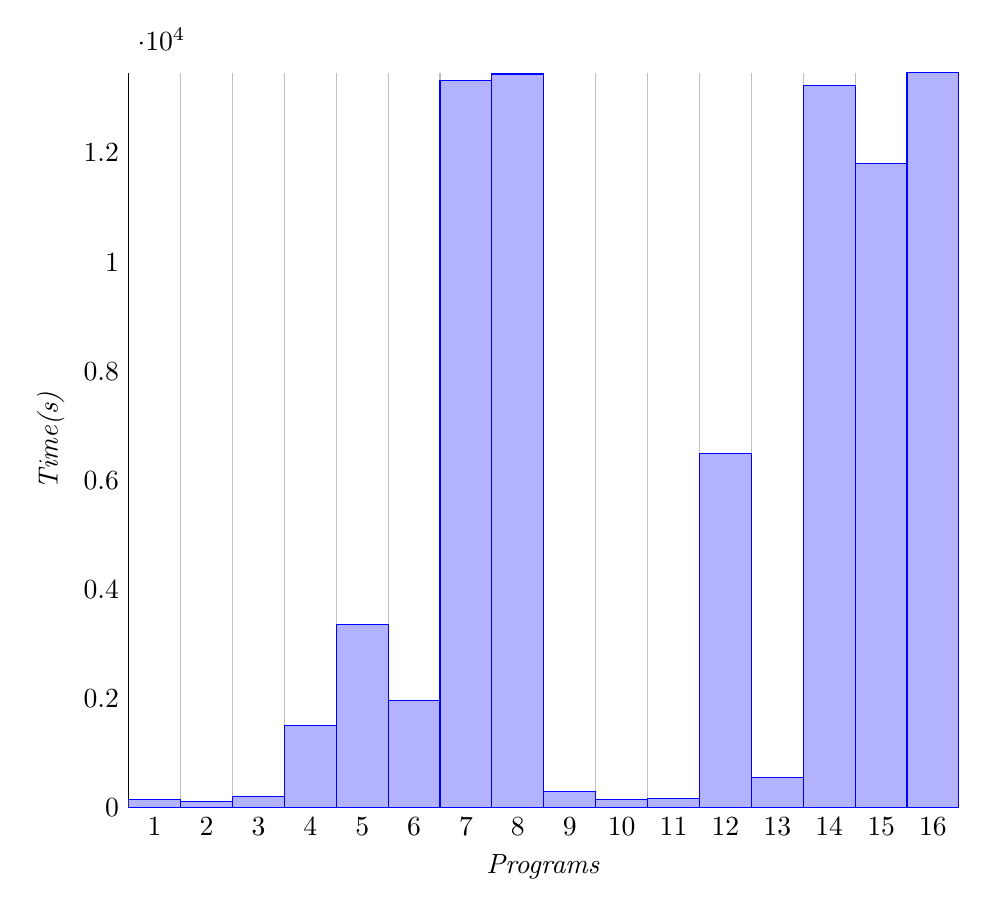
\begin{tikzpicture}
                  \begin{axis}[
                  height = 0.9\textwidth,
                  width = 1\textwidth,
                  ylabel=\emph{Time(s)},
                  xlabel=\emph{Programs},
                  legend style={at={(0.5,-0.2)},cells={align=left},
                  anchor=north,legend columns=1},
                  ybar interval = 1,
                  axis lines=left, % remove top and right axis lines
                  tick align=inside, % move ticks inside the plot area
                  xtick align=inside,
                  axis line style={-}, % remove arrow heads from axes
                  xtick style={draw=none}, % remove ticks
                  ytick style={draw=none},
                  enlarge x limits=false, % don't extend x limits beyond the data range
                  ymajorgrids=false, % remove y grid lines
                  legend style={draw=none}, % remove border from legend
                  ]
                  %Model Ouput
                  \addplot
                  coordinates {
                  (16,13471.964629)
                  (15,11808.325128)
                  (14,13243.207864)
                  (13,551.798543)
                  (12,6483.945198)
                  (11,163.094611)
                  (10,142.0037)
                  (9,300.228418)
                  (8,13449.994491)
                  (7,13328.27705)
                  (6,1969.828764)
                  (5,3351.88337)
                  (4,1500.01275)
                  (3,196.948547)
                  (2,103.677106)
                  (1,139.825496)
                  (0,0)
                  };

                  \end{axis}
            \end{tikzpicture}
      }
      \caption{Waktu Pelatihan Model}
      \label{tb:HasilPengujianTrainTime}
\end{figure}
  

\begin{longtable}{|l|r|r|r|r|r|r|r|}
      \caption{Waktu Generasi Data.}
      \label{tb:HasilPengujianGenTime} \\
      \hline
      \rowcolor[HTML]{C0C0C0}
      \textbf{Program} & \textbf{1\%} & \textbf{2\%} & \textbf{5\%} & \textbf{10\%} & \textbf{25\%} & \textbf{50\%} & \textbf{Per Row Time (s)} \\
      \hline
      Age Analysis & 1 & 2 & 5 & 10 & 24 & 47 & 0.12 \\
      \hline
      Commute Type & 1 & 2 & 3 & 6 & 15 & 30 & 0.14 \\
      \hline
      Commute T-F & 2 & 3 & 7 & 14 & 35 & 69 & 0.45 \\
      \hline
      Customers & 11 & 21 & 53 & 105 & 261 & 522 & 0.05 \\
      \hline
      Delays & 26 & 51 & 126 & 251 & 627 & 1254 & 0.04 \\
      \hline
      Delivery Faults & 16 & 32 & 78 & 156 & 390 & 780 & 0.04 \\
      \hline
      External Call & 100 & 200 & 500 & 1000 & 2500 & 5000 & 0.007 \\
      \hline
      Find Salary & 100 & 200 & 500 & 1000 & 2500 & 4999 & 0.007 \\
      \hline
      Flight Distance & 3 & 5 & 12 & 23 & 57 & 113 & 0.28 \\
      \hline
      Income Agg. & 1 & 2 & 5 & 10 & 25 & 49 & 0.10 \\
      \hline
      Inside Circle & 2 & 3 & 7 & 13 & 32 & 63 & 0.06 \\
      \hline
      Loan Type & 48 & 95 & 238 & 475 & 1187 & 2373 & 0.03 \\
      \hline
      Movie Rating & 5 & 9 & 22 & 44 & 110 & 220 & 0.06 \\
      \hline
      Number Series & 98 & 195 & 487 & 974 & 2434 & 4867 & 0.01 \\
      \hline
      Student Grade & 90 & 179 & 448 & 895 & 2238 & 4475 & 0.01 \\
      \hline
      Word Count & 100 & 200 & 500 & 1000 & 2500 & 5000 & 0.007 \\
      \hline
\end{longtable}
